\section{PyTorch Fuzzing}

PyTorch is a popular open-source machine-learning framework that has gained immense popularity in recent years. Developed by Meta (formerly Facebook), PyTorch has emerged as one of the most widely used machine learning frameworks due to its ease of use, flexibility, and dynamic computational graph, making it a popular choice for researchers and developers alike.

PyTorch is a critical component of many applications across various industries such as banking, healthcare, insurance, and many others. It is used for natural language processing, image classification, speech recognition, and other tasks. In banking, PyTorch is used to develop fraud detection systems, while in healthcare, it is used to diagnose diseases and predict patient outcomes. The insurance industry uses PyTorch to analyze risk and predict losses. The flexibility of PyTorch enables it to be used in many other domains as well. PyTorch has been used to build many state-of-the-art machine learning models and is a vital tool in the field of deep learning.

Despite its popularity and usefulness, PyTorch has several challenges that must be addressed to ensure its reliability and security. PyTorch has multiple dependencies, and it includes a considerable amount of C/C++ code which implies that it is susceptible to memory safety vulnerabilities. Moreover, PyTorch is an interesting target for adversaries since it is used in critical applications. Therefore, it is crucial to ensure that PyTorch is secure and free from vulnerabilities. Fuzzing is a valuable technique that can help identify bugs and vulnerabilities in PyTorch, making it more robust and secure. By fuzzing PyTorch, we can ensure that it can withstand attacks and continue to operate correctly in real-world applications.

This chapter delves into the concept of PyTorch fuzzing and its importance in enhancing the reliability and security of PyTorch. The exploration commences with an examination of its attack surface. Subsequently, fuzzing harnesses will be developed for the relevant sections of the codebase. The fuzzing methodology and the outcomes of the work will be outlined as well.

\subsection{Attack Surface Mapping}

To initiate the fuzzing process, it is essential to determine the attack surface of PyTorch. The attack surface refers to all the entry points through which an attacker can potentially interact with the system and launch an attack. In the case of PyTorch, its attack surface includes various modules, libraries, and dependencies that it uses.

To identify interesting parts of the codebase that are relevant to the attack surface, a manual code analysis was conducted. This analysis has highlighted several modules that are particularly interesting to analyze, including the model loading and RPC communications modules.

\subsubsection{Model Loading}

The process of loading pre-trained models is a crucial entry point that attackers can exploit to gain access to the system. This process is typically handled by the model loading module, which can be accessed via the \texttt{torch.load()} function.

During the loading process, the \texttt{torch.load()} function goes through several deserialization steps, also known as unpickling, to recreate the original object from the byte stream. Deserialization is a common source of vulnerabilities in many applications, as it can be difficult to implement correctly. Unfortunately, PyTorch is not immune to this issue. Additionally, since the implementation is written in C++, it is even more susceptible to memory safety vulnerabilities.

The code responsible for model loading and parsing is mostly located in these files:

\begingroup
\begin{itemize}
    \item jit/serialization/import.cpp
    \item jit/ir/irparser.cpp
    \item jit/serialization/unpickler.cpp
    \item jit/runtime/interpreter.cpp
    \item jit/frontend/schema\_type\_parser.cpp
\end{itemize}
\endgroup

\subsubsection{Remote Communications (RPC)}

Besides model loading, PyTorch has another interesting mechanism that attackers can exploit - the RPC communications module.

The RPC module in PyTorch is a complex system that opens up new, remotely accessible attack vectors. PyTorch uses the RPC module to implement distributed training and inference that allows users to train and execute models across multiple machines. This feature is essential for large-scale applications that require high computational power. However, it increases the security risks by creating additional entry points for attackers.

PyTorch uses various types of RPCs such as \texttt{RRef} (Remote Reference),\\ \texttt{ScriptCall}, and others to interact with remote machines. Before sending RPCs, they are serialized into pickled objects using the \texttt{torch::jit::pickle} function. The RPCs are then sent using different backends like TensorPipe, Gloo, and MPI. Once received, the RPCs are deserialized using the \texttt{torch::jit::unpickle} function, and the target \texttt{Message}'s class \texttt{fromMessage()} method is called. This leaves the receiver with a plain message that can be further processed.

Unfortunately, the complexity of this system makes it prone to bugs and vulnerabilities. Multiple serializations and deserializations of messages can introduce bugs, and the fact that the RPC protocol is implemented in C++ makes it an attractive target to look for memory safety vulnerabilities. Moreover, given the memory-unsafe nature of the RPC protocol, a single bug could potentially allow an attacker to execute code remotely on a target machine. As a result, fuzzing the RPC module is highly recommended to identify and address potential vulnerabilities.

Taking that into consideration, the following files have been identified as the most interesting targets for security research.

\begingroup
\begin{itemize}
    \item distributed/rpc/*.cpp
    \item jit/serialization/unpickler.cpp
\end{itemize}
\endgroup

\subsubsection{Finding Fuzz-Targets}

Having identified various sections of the PyTorch codebase that are relevant to the attack surface, we can proceed to the second part of the attack surface mapping - identifying specific functions and methods to fuzz.

To achieve this, two different approaches have been used:

\begin{enumerate}
    \item \textbf{Manual code review} - A manual code review of the PyTorch codebase has been performed to identify relevant functions that are confined to the defined attack surface.
    \item \textbf{CodeQL} - A CodeQL \cite{ql-object-oriented-queries-on-relational-data} has been utilized to broadly search for interesting functions and methods that perform some kind of deserialization or parsing.
\end{enumerate}

The first approach is straightforward and does not require any additional tools. However, it is time-consuming and requires a lot of manual work. Nevertheless, it yields the best results since it allows a researcher to precisely identify the functions that might be interesting to fuzz.

The second approach lacks "precision" but can be automated and scaled to a large codebase. It allows for quick identification of a narrowed-down set of functions that are worth looking into. However, it is not as precise as the first approach since it relies on heuristics and does not "understand" the code. As a result, it can miss some relevant functions. Nevertheless, it is a good starting point for fuzzing since it can help identify interesting functions that can be further analyzed manually.

To begin with, the second approach was employed to pinpoint some specific functions that are worth looking into. A CodeQL query \ref{appendix:codeql-query} was developed to search for functions that have two parameters:

\begin{enumerate}
    \item The first parameter is a pointer to data of "parsable" types. For example - \texttt{char*}, \texttt{byte*}, and others.
    \item The second parameter is an integer that represents the size of the data. For example - \texttt{int}, \texttt{size\_t}, and others.
\end{enumerate}

With that in place, a few more heuristics were added to filter out irrelevant functions. Finally, \textit{Cyclomatic Complexity} \cite{cyclomatic-complexity-density} was used to rank the results and identify the most complex functions. Some results of the query are shown in Table \ref{table:codeql-results}.

\begin{table}[h]
    \centering
    \begin{tabular}{cl}
        \toprule
        \textbf{Complexity} & \textbf{Function}                      \\
        13                  & \texttt{rpc::parseWireSections}        \\
        6                   & \texttt{Unpickler::readSlowWithBuffer} \\
        5                   & \texttt{TokenTrie::insert}             \\
        4                   & \texttt{rpc::wireDeserialize}          \\
        \bottomrule
    \end{tabular}
    \caption{CodeQL query results}
    \label{table:codeql-results}
\end{table}

These findings served as a solid starting point. From here, the functions were manually reviewed, and the codebase was thoroughly studied, employing the first approach.

Finally, a list of the most interesting functions that are worth fuzzing has been compiled. The list is shown in Table \ref{table:fuzz-targets}.

\begin{table}[h]
    \centering
    \begin{tabular}{cl}
        \toprule
        \textbf{Function}                 \\
        \texttt{jit::parseIR}             \\
        \texttt{jit::load}                \\
        \texttt{rpc::deserializeResponse} \\
        \texttt{rpc::deserializeRequest}  \\
        \bottomrule
    \end{tabular}
    \caption{Fuzz targets}
    \label{table:fuzz-targets}
\end{table}

The first two functions are related to the JIT module and are responsible for parsing and loading the pickled data. Some examples of such data are: \texttt{saved models}, \texttt{serialized requests}, and others.

The last two functions are related to the RPC module and are responsible for deserializing RPC requests and responses. These functions are interesting because they are directly processing untrusted data that is received from the network.

Besides that, another interesting function - \texttt{jit::preoptimizeGraph}, has been identified within the JIT module. It has been chosen as a target for differential fuzzing, with the objective of uncovering bugs associated with JIT graph optimizations.

\subsection{Preparing PyTorch for Fuzzing}

Having identified the fuzz targets, the subsequent step involves the development of a fuzzing harness. The goal of the fuzzing harness is to provide a way to feed the fuzz target with data and collect the results of the execution. In alignment with the chosen objective, \textit{LibFuzzer}-compatible \cite{libfuzzer-secdev-2016} targets have been created for each of the functions enumerated in Table \ref{table:fuzz-targets}.

Each libFuzzer-based target shares the same structure. The structure is shown in Listing \ref{listing:fuzz-target-structure}.

\begin{listing}[h]
    \centering
    \begin{minipage}{.9\linewidth}
        \begin{minted}[linenos=true, tabsize=4]{cpp}
int LLVMFuzzerTestOneInput(const uint8_t* data, size_t size) {
    // 1. Prepare the input data
    // 2. Call the fuzz target with the parsed data
    // 3. Return 0
}
    \end{minted}
    \end{minipage}
    \caption{Fuzz target structure}
    \label{listing:fuzz-target-structure}
\end{listing}

The goal of a generic fuzzing harness is to pass the data generated by the fuzzer to the fuzz target and clean up the resources after the execution is finished. The fuzzing harness is also responsible for handling the exceptions that might be thrown by the fuzz target.

The fuzzing harnesses that have been developed for PyTorch are similar to the generic one. However, they also perform some additional steps. For example, they handle some PyTorch-specific exceptions.

The developed fuzzing harnesses are listed below:

\begin{itemize}
    \item \href{https://github.com/ispras/oss-sydr-fuzz/blob/028e36875424aec00ef7375006c413a4be164197/projects/pytorch/irparser_fuzz.cc}{\texttt{irparser\_fuzz.cc}} - fuzzes \texttt{jit::parseIR}
    \item \href{https://github.com/ispras/oss-sydr-fuzz/blob/028e36875424aec00ef7375006c413a4be164197/projects/pytorch/load_fuzz.cc}{\texttt{load\_fuzz.cc}} - fuzzes \texttt{jit::load}
    \item \href{https://github.com/ispras/oss-sydr-fuzz/blob/028e36875424aec00ef7375006c413a4be164197/projects/pytorch/message_deserialize_fuzz.cc}{\texttt{message\_deserialize\_fuzz.cc}} - fuzzes \texttt{rpc::deserializeResponse} and \texttt{rpc::deserializeRequest}
    \item \href{https://github.com/ispras/oss-sydr-fuzz/blob/028e36875424aec00ef7375006c413a4be164197/projects/pytorch/jit_differential_fuzz.cc}{\texttt{jit\_differential\_fuzz.cc}} - fuzzes three related methods - \texttt{jit::parseIR}, \texttt{jit::preoptimizeGraph}, and \texttt{jit::InterpreterState(code).run()} with differential fuzzing
\end{itemize}

However, the development of fuzzing harnesses is only one more step on the road toward hybrid fuzzing. The next step is to compile all the necessary build targets.

\newparagraph{LibFuzzer Target}

The first one is the fuzz target itself. It is the main entry point for the fuzzer. This target is compiled using the \textit{clang} compiler with the \textit{libFuzzer} library linked, as well as the \textit{libasan} library. The latter is known as the \textit{AddressSanitizer} \cite{address-sanitizer-usenix-2012} and is required to maximize the chances of finding memory-related bugs.

To build this target, the following compilation flags were added to the build script: \texttt{-fPIC -g -fsanitize=fuzzer,address,bounds}. To easily distinguish the produced binary from other targets, a \texttt{\_fuzz} suffix was added to its name.

\newparagraph{Sydr Target}

The second type of build target is the plain binary for symbolic execution, which reads the data directly from the file and passes it to the fuzz target, without involving the fuzzer. It allows the symbolic execution engine to execute the fuzz target with concrete data. This target is also compiled with the help of the \textit{clang} compiler, however, the flags are different: \texttt{-fPIC -g}. Moreover, this time sanitizers are not used, as they would only complicate the symbolic execution process. A \texttt{\_sydr} suffix was also added to the name of the binary.

\newparagraph{Coverage Target}

And the last type of build target is the binary that is used to collect the coverage information. It is compiled with the \textit{clang} compiler and the following flags: \texttt{-fPIC -g -fprofile-instr-generate -fcoverage-mapping}. As for the previous targets, the \texttt{\_cov} suffix has been incorporated into the binary's name.

\subsection{PyTorch Hybrid Fuzzing}

With all the artifacts produced, we can now proceed to the next step - hybrid fuzzing. The goal of this step is to prepare the corpus, perform the fuzzing, and analyze the results. To carry out hybrid fuzzing, the \textit{sydr-fuzz} tool, developed by ISP RAS, has been employed. The \textit{sydr-fuzz} framework is a versatile tool for hybrid fuzzing, enabling the seamless integration of symbolic execution engines and state-of-the-art fuzzers like \textit{AFL++} and \textit{libFuzzer} for efficient fuzzing of the target program.

\subsubsection{Preparing the Corpus}

Prior to commencing the fuzzing, it is necessary to prepare the corpus for the fuzzer. The corpus represents a collection of inputs that the fuzzer utilizes to generate new inputs.

As most of the targets were aimed at fuzzing the unpickling functionality, the corpus was gathered by extracting test models from the PyTorch repository. Besides unpickling, a few targets were aimed at fuzzing the IR-parsing functionality. For these targets, tests that use the \texttt{jit::parseIR} method were found and the corresponding intermediate representations (IRs) were extracted. An example of such a test case is shown in Listing \ref{listing:ir-program}.

\begin{listing}[h]
    \centering
    \begin{minipage}{.75\linewidth}
        \begin{minted}[linenos=true, tabsize=4]{cpp}
graph(%a : Tensor):
      %b : Tensor = aten::mul(%a, %a)
      %c : Tensor = aten::mul(%b, %b)
      %d : Tensor = aten::mul(%c, %c)
      %c_size : int[] = aten::size(%c)
      %c_alias : Tensor = aten::view(%c, %c_size)
      %e : Tensor = aten::mul(%b, %d)
      %f : Tensor = aten::mul(%c_alias, %c_alias)
      %output : Tensor = aten::mul(%e, %f)
      return (%output)
    \end{minted}
    \end{minipage}
    \caption{IR program extracted from the PyTorch repository}
    \label{listing:ir-program}
\end{listing}

\subsubsection{Dynamic Analysis Pipeline}

With all the necessary preparations completed, the actual fuzzing process can now be initiated. Fuzzing is carried out through a continuous dynamic analysis pipeline, as depicted in Diagram \ref{fig:dynamic-analysis-pipeline}. This pipeline operates continuously, reflecting the iterative nature of bug-fixing and testing. Whenever a new version of the program is released or a patch is proposed, the pipeline is triggered.

The pipeline consists of the following steps:

\begin{figure}[h]
    \centering
    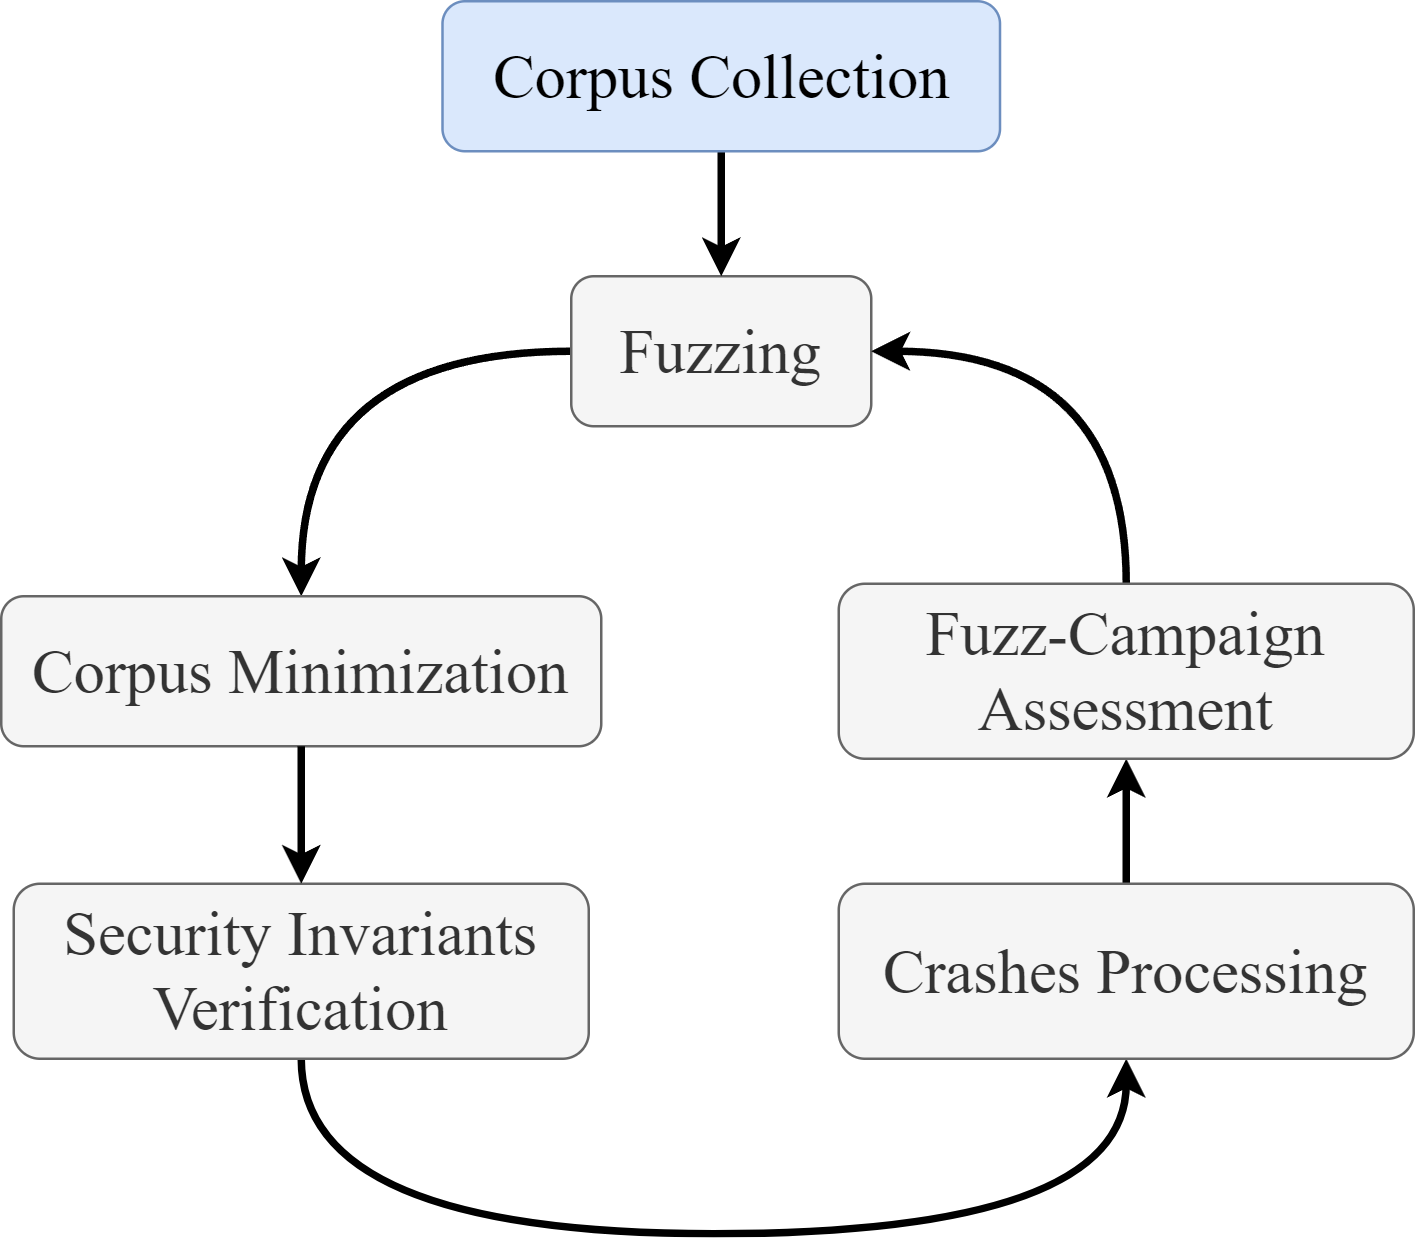
\includegraphics[width=10cm]{assets/dynamic-analysis-pipeline-tnr.png}
    \caption{Dynamic analysis pipeline}
    \label{fig:dynamic-analysis-pipeline}
\end{figure}

\newparagraph{Hybrid Fuzzing}

The first step of the pipeline is hybrid fuzzing. It is performed with the help of the \textit{sydr-fuzz} tool. The tool takes a toml configuration file as input, which specifies the targets to be fuzzed and other parameters. For example, the configuration file for the \texttt{jit\_differential} target is shown in Listing \ref{listing:jit-differential-config}.

\begin{listing}[h]
    \centering
    \begin{minipage}{.75\linewidth}
        \begin{minted}[linenos=true, tabsize=4, breaklines=true]{toml}
[sydr]
args = "-l debug"
target = "/jit_differential_sydr @@"

[libfuzzer]
path = "/jit_differential_fuzz"
args = "-detect_leaks=0 -rss_limit_mb=30720 -timeout=300 -report_slow_units=350 /ir_corpus"

[cov]
target = "/jit_differential_cov @@"
\end{minted}
    \end{minipage}
    \caption{Configuration file for the \texttt{jit\_differential} target}
    \label{listing:jit-differential-config}
\end{listing}

This configuration file contains three sections: \texttt{sydr}, \texttt{libfuzzer}, and \texttt{cov}. The \texttt{sydr} section contains information about the target program and how to execute it under the symbolic execution engine. The \texttt{libfuzzer} section contains libfuzzer-related information, such as the path to the fuzz target binary and the arguments that should be passed to it. Finally, the \texttt{cov} section contains information about the coverage target.

With the configuration file prepared, the fuzzing campaign can be started. To do so, the \textit{sydr-fuzz} binary needs to be executed as follows: \texttt{sydr-fuzz -c jit\_differential.toml run}. The command will start the fuzzing process and will print the results to the console.

\newparagraph{Corpus Minimization}

After running the fuzzer for some time, the subsequent step in the pipeline involves corpus minimization. The goal of this step is to reduce the size of the corpus by removing the redundant inputs. The corpus minimization is performed using the \textit{sydr-fuzz} tool in the \textit{cmin} mode. Under the hood, \textit{sydr-fuzz} uses either \textit{afl-cmin} or the \textit{libfuzzer -merge=1} utilities.

This step is optional, however, it is highly recommended, because it greatly improves the performance of the next step - security invariants verification. Without corpus minimization, the security invariants verification is less likely to find any bugs, as it will potentially re-execute almost the same inputs multiple times.

\newparagraph{Security Invariants Verification}

The next step of the pipeline is security invariants verification. The idea behind this step is to execute the \textit{sydr} symbolic execution engine in the \textit{security} mode, with inputs from the minimized corpus. The \textit{security} mode is a special mode that is designed to check for violation of various security invariants, such as integer overflows, null pointer dereferences, buffer overflows, and others. If any of the invariants are violated, the symbolic execution engine will report the corresponding bug.

Running the symbolic execution engine in the \textit{security} mode is a very expensive operation. For this reason, efforts have been directed toward optimizing its performance. The results are discussed in chapter \ref{hybrid-fuzzer-improvements:optimizing-security-predicates}.

\newparagraph{Crashes Processing}

Near the end, the crashes processing is performed. During previous steps, \textit{sydr-fuzz} may have found some crashes. At this stage, those crashes need to be deduplicated and preprocessed. To do so, \textit{sydr-fuzz} employs the \textit{casr} tool \cite{casr-cluster-ispras-2021}. This tool performs automatic crashes processing, which includes deduplication, and clusterization.

Executing \textit{sydr-fuzz} in this mode, using the following command: \texttt{sydr-fuzz -c jit\_differential.toml casr}, will produce a set of processed crashes.
\newparagraph{Fuzz-Campaign Assessment}

Finally, after all the steps are completed, the results of the fuzzing campaign are assessed. The assessment is performed manually by the user, and includes the following steps:

\begin{enumerate}
    \item Bug triaging and reporting
    \item Code coverage analysis
\end{enumerate}

During the bug triaging and reporting step, the user needs to analyze the found bugs and decide whether they are real bugs or not. If the bug is proven to be real, the user needs to report it to the developers of the target program.

The code coverage analysis step is performed to assess the effectiveness of the fuzzing campaign. The goal of this step is to help the user to understand whether the fuzzing campaign was effective and whether it is worth continuing it. The code coverage analysis is performed using the \textit{sydr-fuzz} tool in the \textit{cov} mode.

This concludes the description of the dynamic analysis pipeline, which has been used to fuzz the PyTorch framework. In the next section, some of the findings will be discussed.

\subsection{Results Overview}

As a result of this work, multiple bugs were found in different parts of the PyTorch framework. The majority of the bugs were discovered within the module responsible for unpickling. Nevertheless, it is worth noting that at least one remotely-accessible bug was identified in the RPC module.

All discovered bugs were reported to the PyTorch framework developers, who confirmed their validity and subsequently merged the corresponding pull requests into the PyTorch repository. The pull requests related to the bugs are listed below:

\begin{itemize}
    \item \href{https://github.com/pytorch/pytorch/pull/94300}{\#94300: Add size check before calling stack\_.at(dict\_pos) in unpickler.cpp}
    \item \href{https://github.com/pytorch/pytorch/pull/94298}{\#94298: Add stack emptiness checks inside interpreter.cpp}
    \item \href{https://github.com/pytorch/pytorch/pull/94297}{\#94297: Add size check before calling .back() in rpc/script\_call.cpp}
    \item \href{https://github.com/pytorch/pytorch/pull/94295}{\#94295: Add exception handlers for stoll in schema\_type\_parser.cpp}
    \item \href{https://github.com/pytorch/pytorch/pull/91401}{\#91401: Add out-of-bounds checks inside irparser.cpp and unpickler.cpp}
\end{itemize}

In section \ref{results:pytorch-findings}, a closer inspection of the bugs found, and the pull created will be performed.
